\section{PKSTU}
\begin{frame}{彭康学导团现有的以\LaTeX 排版的资料}
    \begin{itemize}
        \item 大学物理(上)笔记 \link{https://github.com/PKSTU/University-Physics-Notes.git}
        \begin{columns}
            \begin{column}{0.48\textwidth}
                \begin{figure}
                    \centering
                    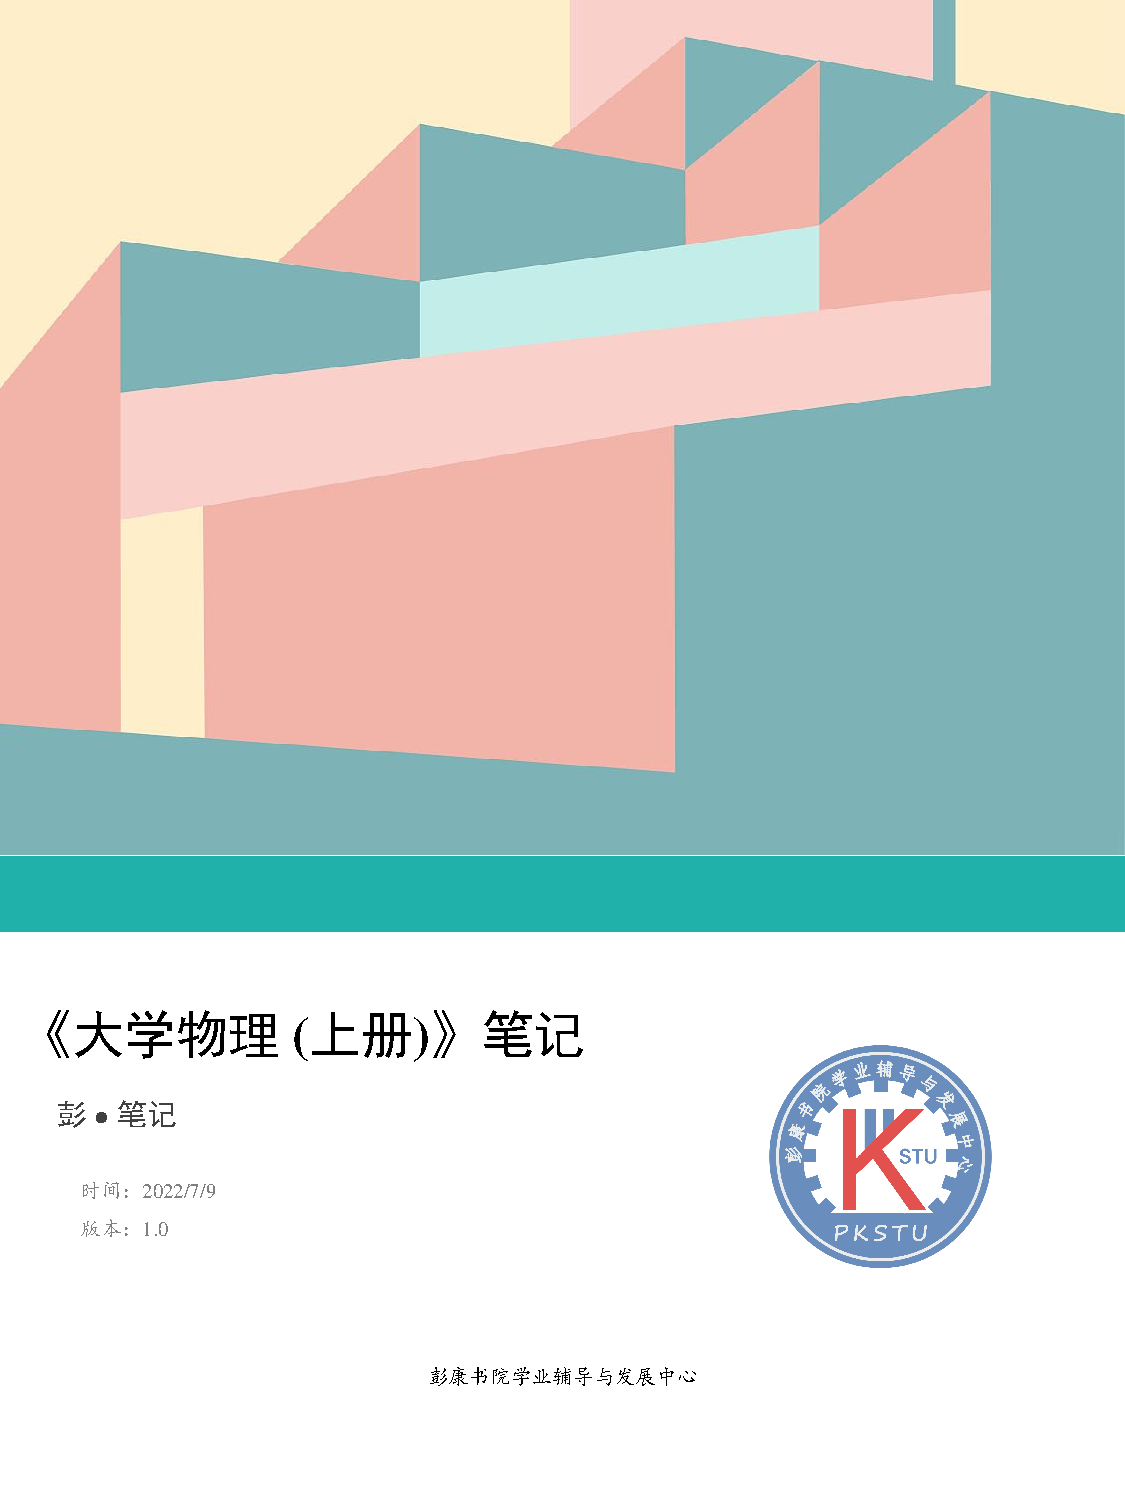
\includegraphics[scale=0.2]{figures/PK_DW1.pdf}
                \end{figure}
            \end{column}
            \begin{column}{0.48\textwidth}
                \begin{figure}
                    \centering
                    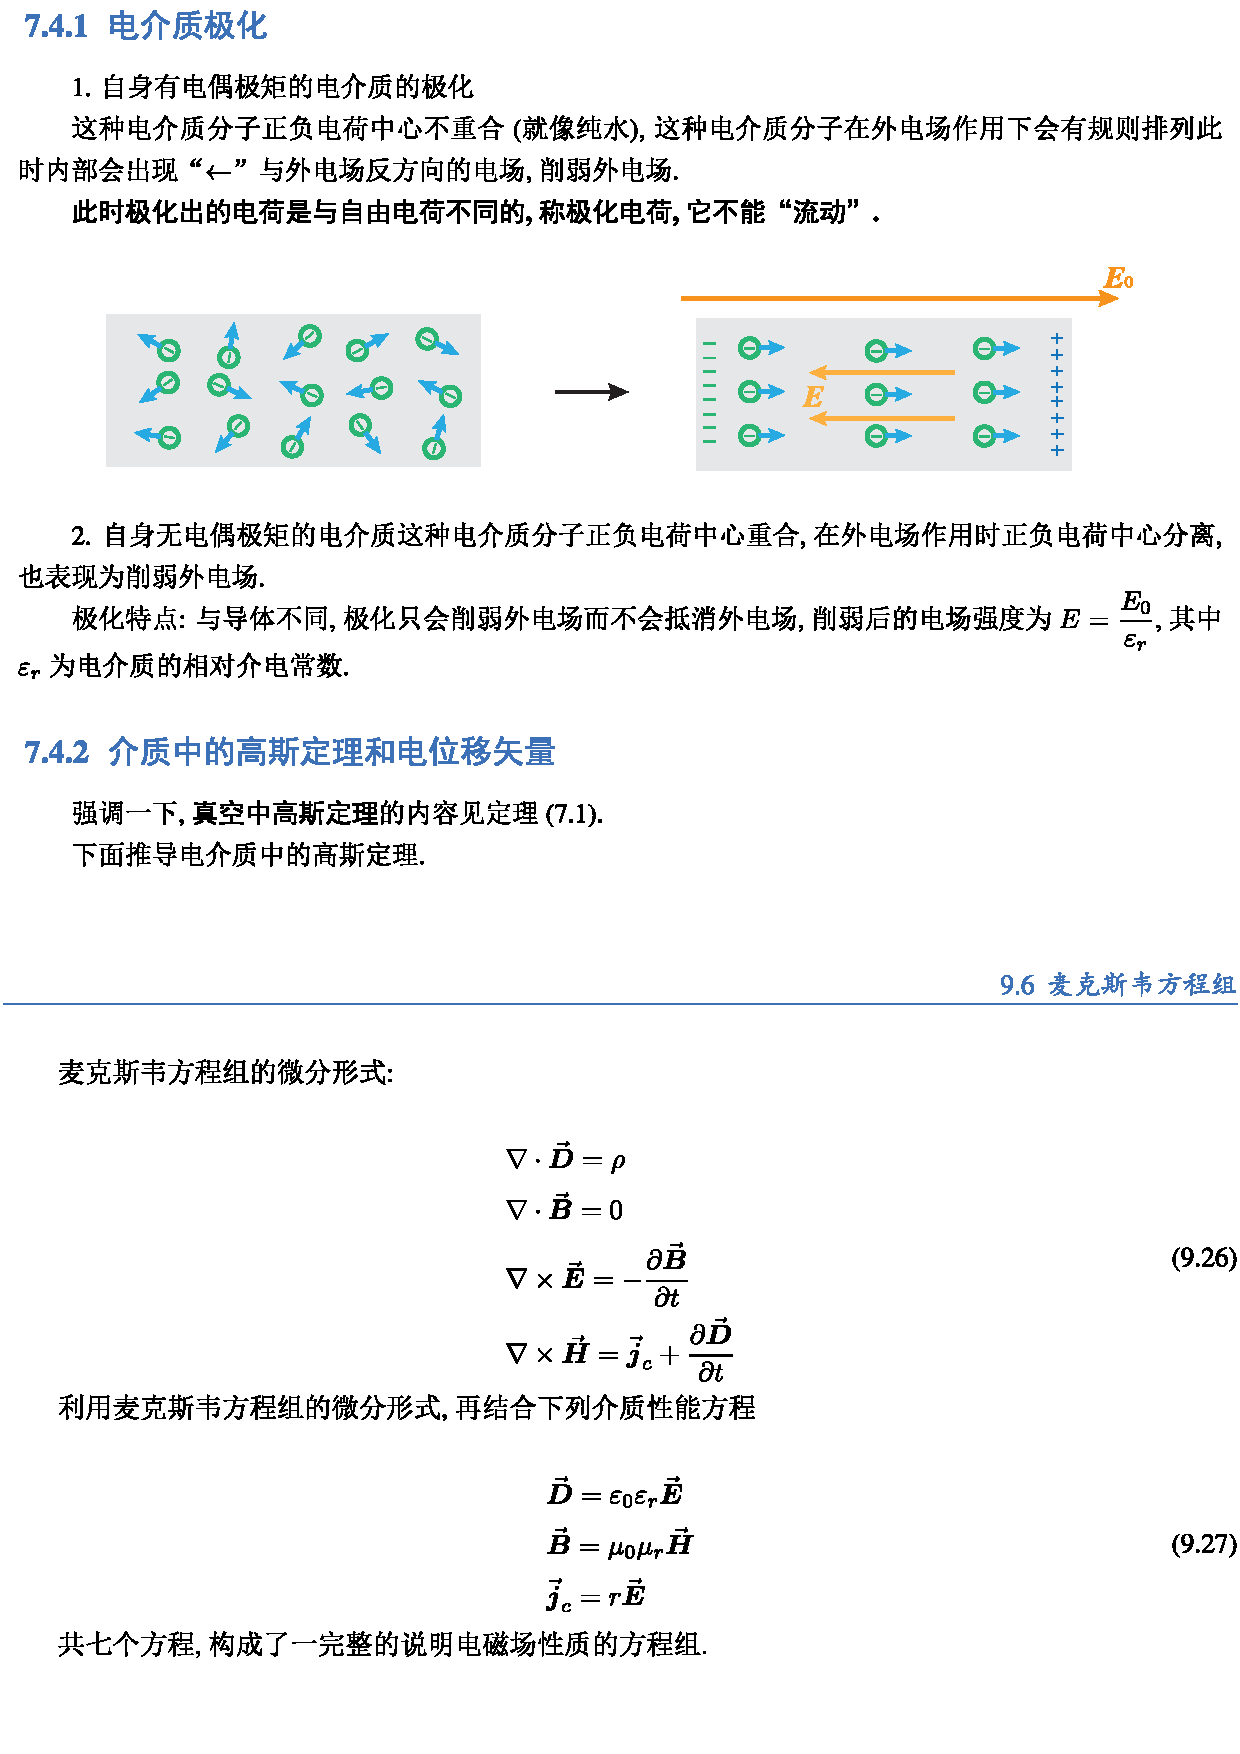
\includegraphics[scale=0.2]{figures/PK_DW2.pdf}
                \end{figure}
            \end{column}
        \end{columns}
    \end{itemize}
\end{frame}

\begin{frame}{彭康学导团现有的以\LaTeX 排版的资料}
    \begin{itemize}
        \item 高等数学(上)\& 线性代数入门讲义 \link{https://github.com/PKSTU/Advanced-Mathematics-Notes.git} \link{https://github.com/PKSTU/Linear-Algebra-Notes.git}
        \begin{columns}
            \begin{column}{0.48\textwidth}
                \begin{figure}
                    \centering
                    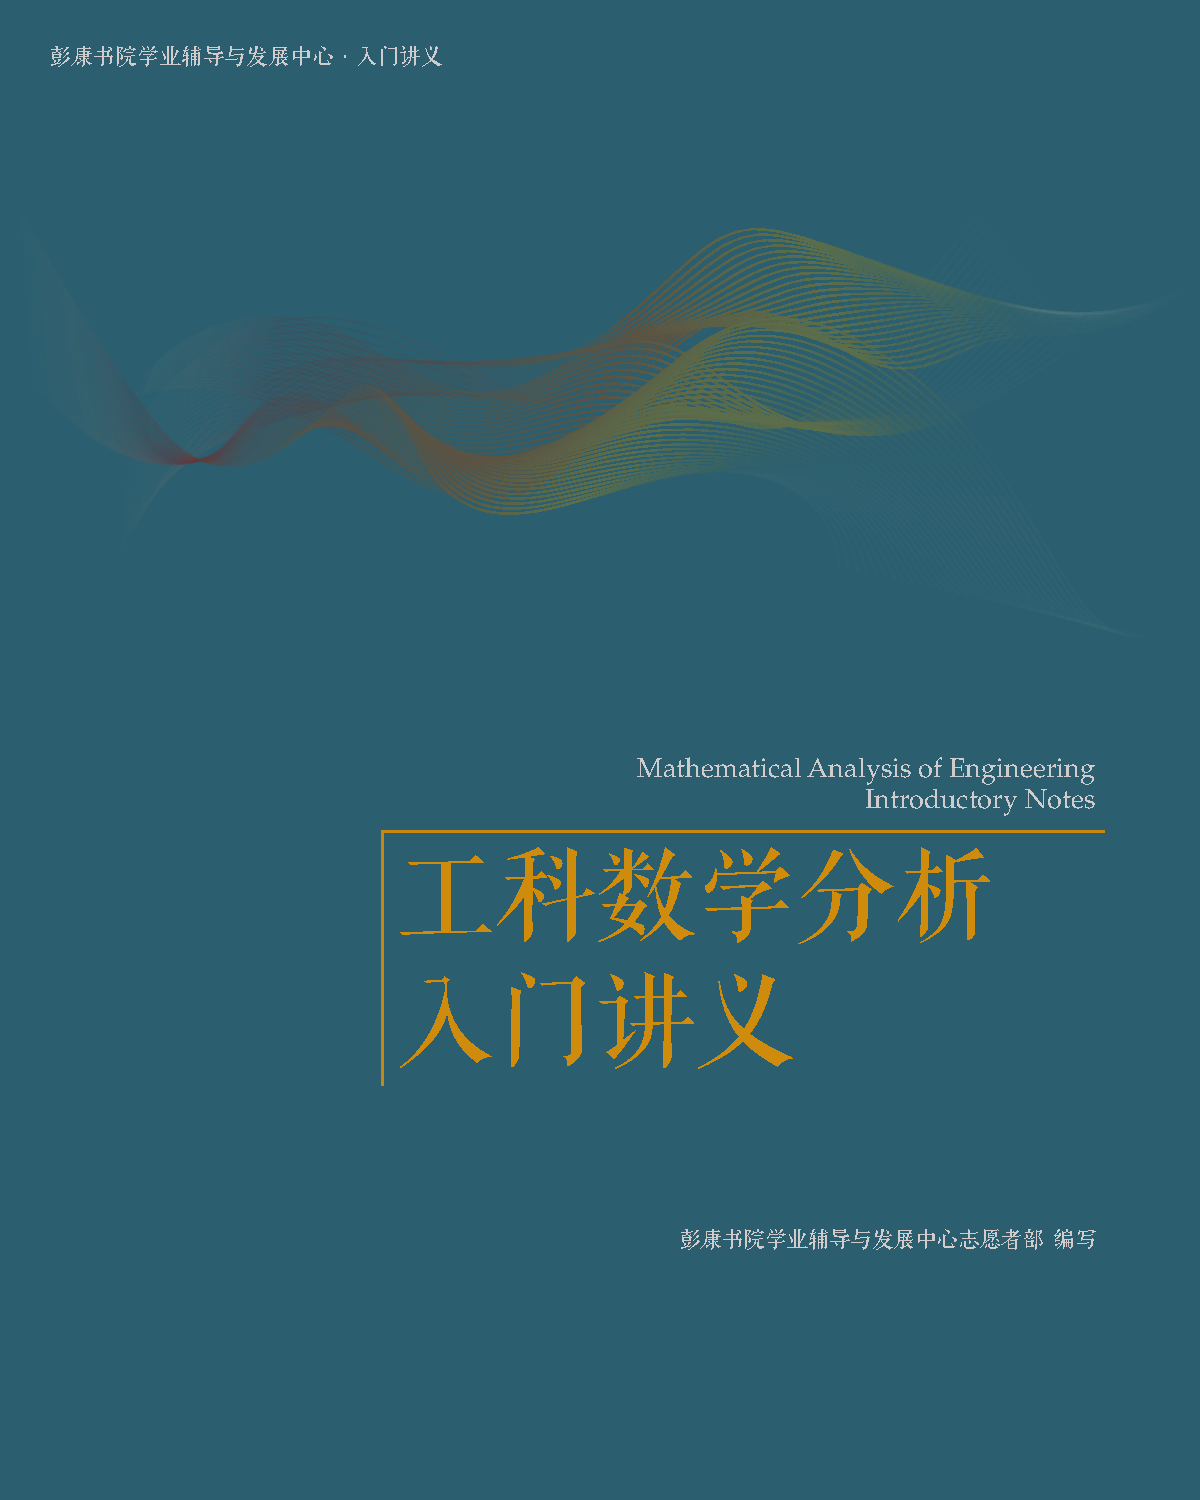
\includegraphics[scale=0.2]{figures/PK_GS.pdf}
                \end{figure}
            \end{column}
            \begin{column}{0.48\textwidth}
                \begin{figure}
                    \centering
                    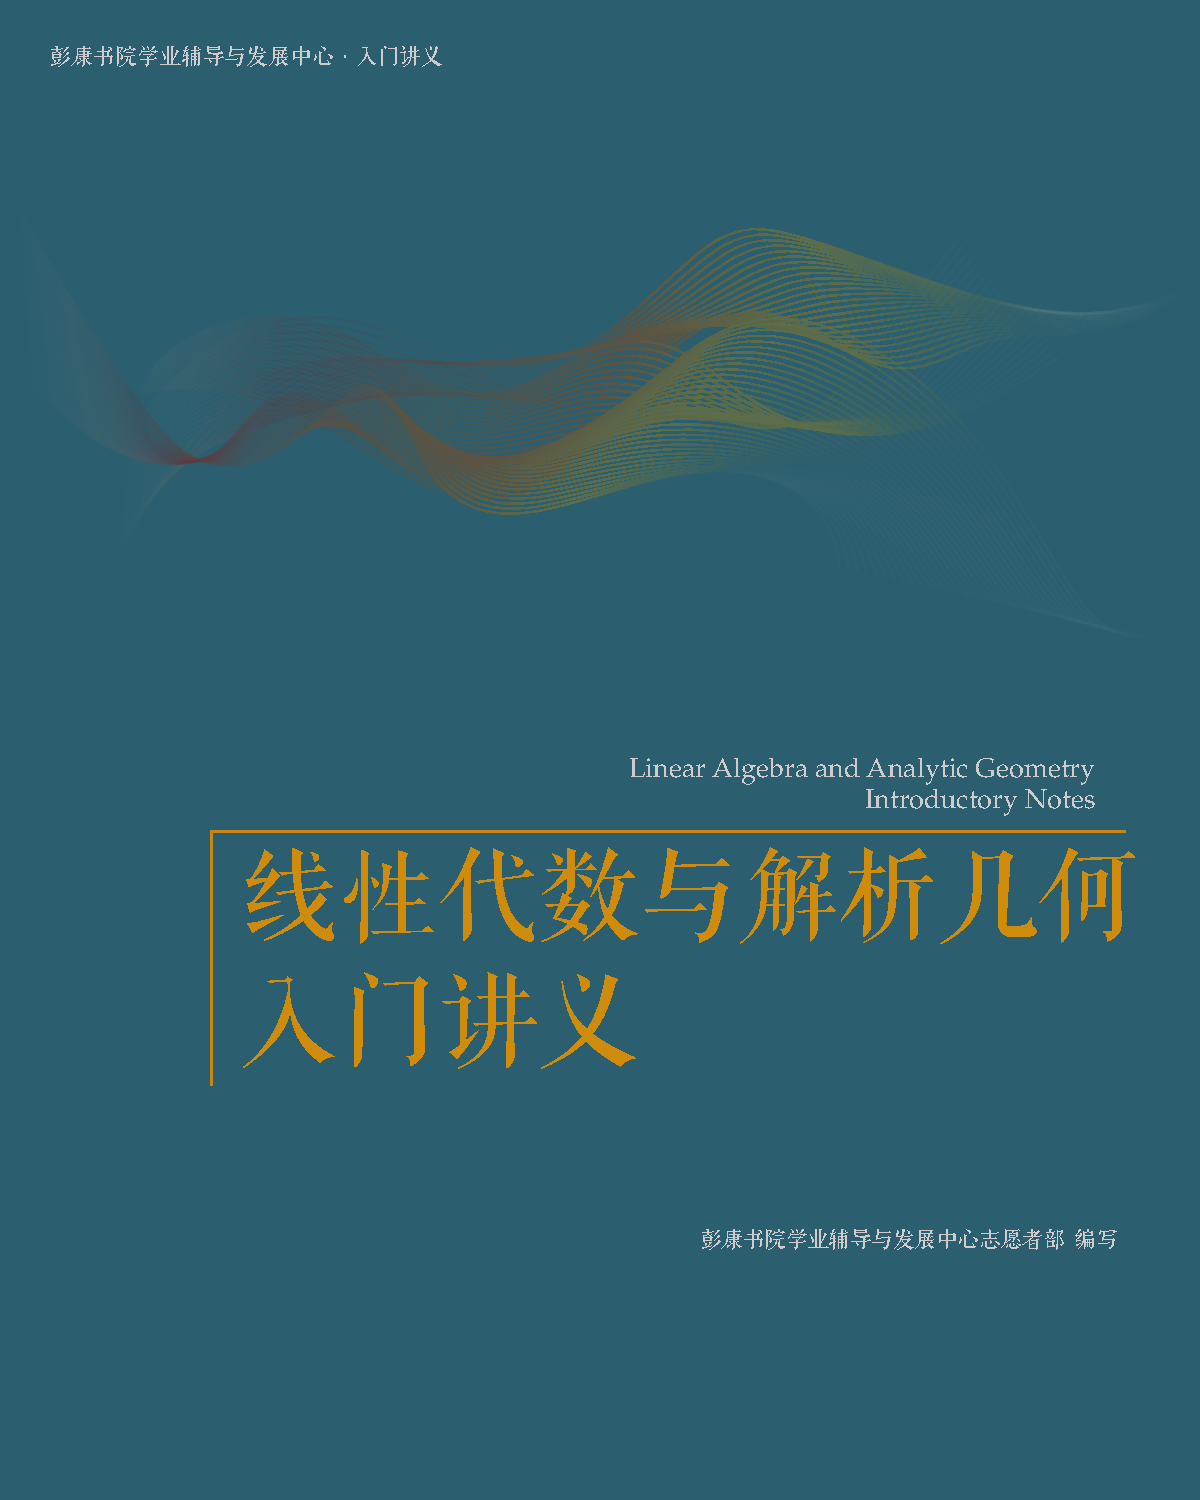
\includegraphics[scale=0.2]{figures/PK_XD.pdf}
                \end{figure}
            \end{column}
        \end{columns}
    \end{itemize}
\end{frame}

\begin{frame}{彭康学导团现有的以\LaTeX 排版的资料}
    \begin{itemize}
        \item 流体力学复习要点 \link{https://github.com/PKSTU/Hydrodynamics-Key-Points.git}
        \begin{columns}
            \begin{column}{0.48\textwidth}
                \begin{figure}
                    \centering
                    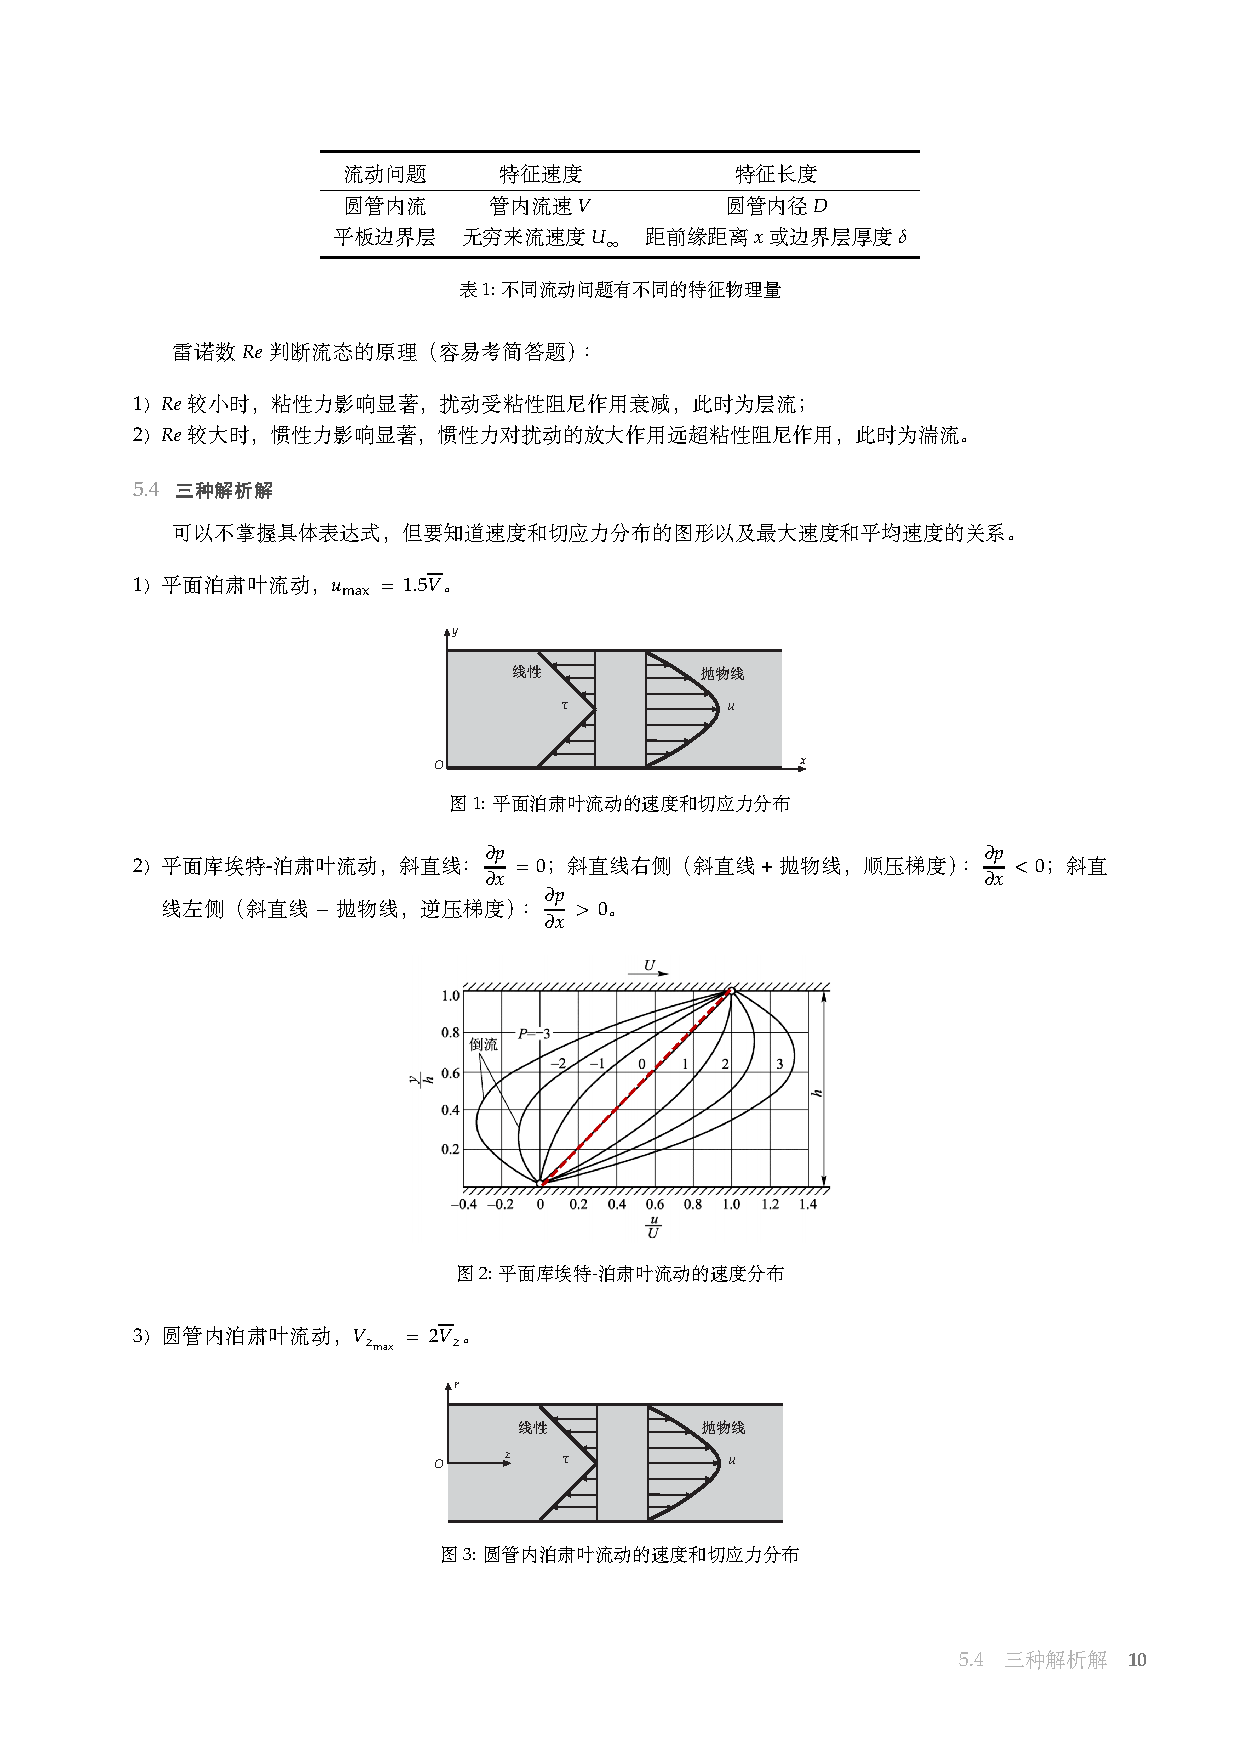
\includegraphics[scale=0.2]{figures/PK_LL1.pdf}
                \end{figure}
            \end{column}
            \begin{column}{0.48\textwidth}
                \begin{figure}
                    \centering
                    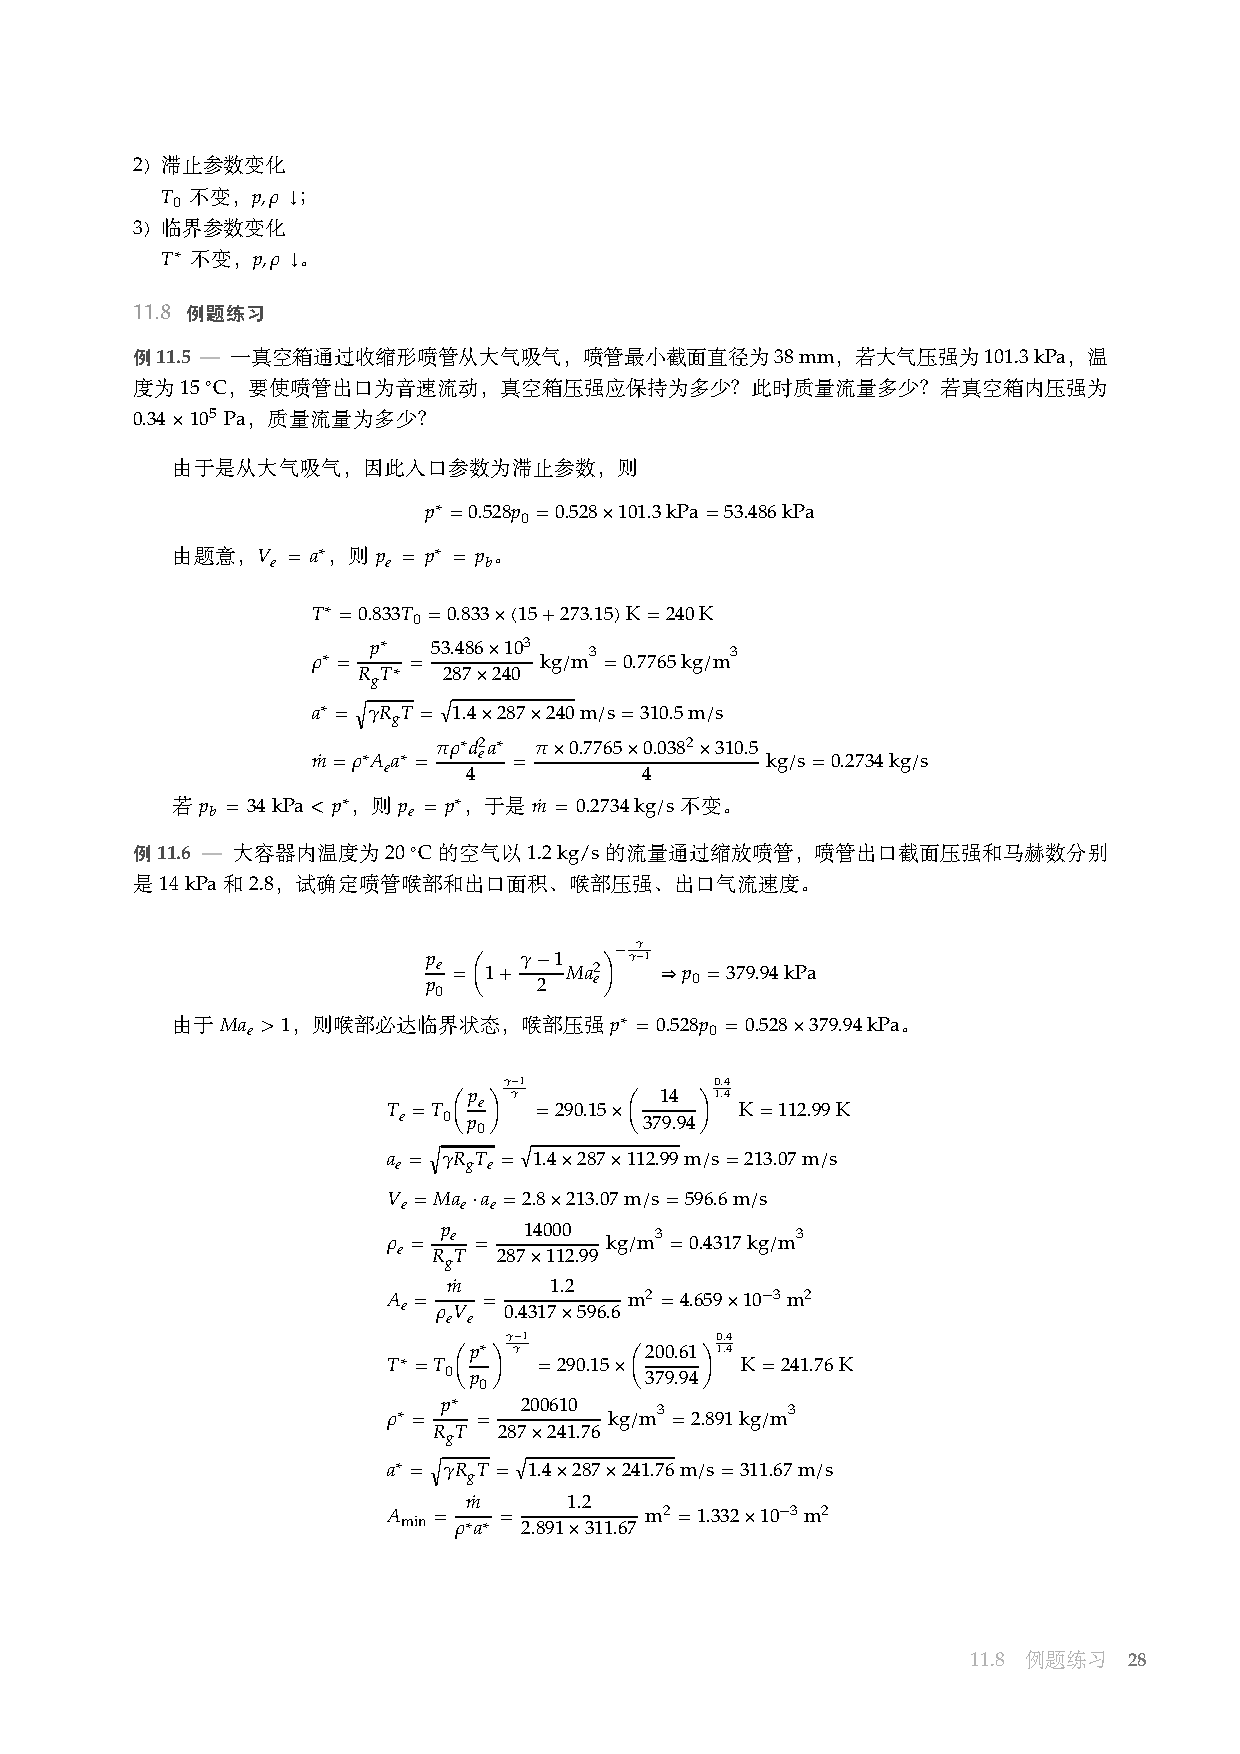
\includegraphics[scale=0.2]{figures/PK_LL2.pdf}
                \end{figure}
            \end{column}
        \end{columns}
    \end{itemize}
\end{frame}

\begin{frame}{彭康学导团现有的以\LaTeX 排版的资料}
    \begin{itemize}
        \item 最新的高数、线代真题及解析 \link{https://github.com/PKSTU/PKSTU-Exam-Advanced-Mathematics-Linear-Algebra.git}
        \begin{columns}
            \begin{column}{0.48\textwidth}
                \begin{figure}
                    \centering
                    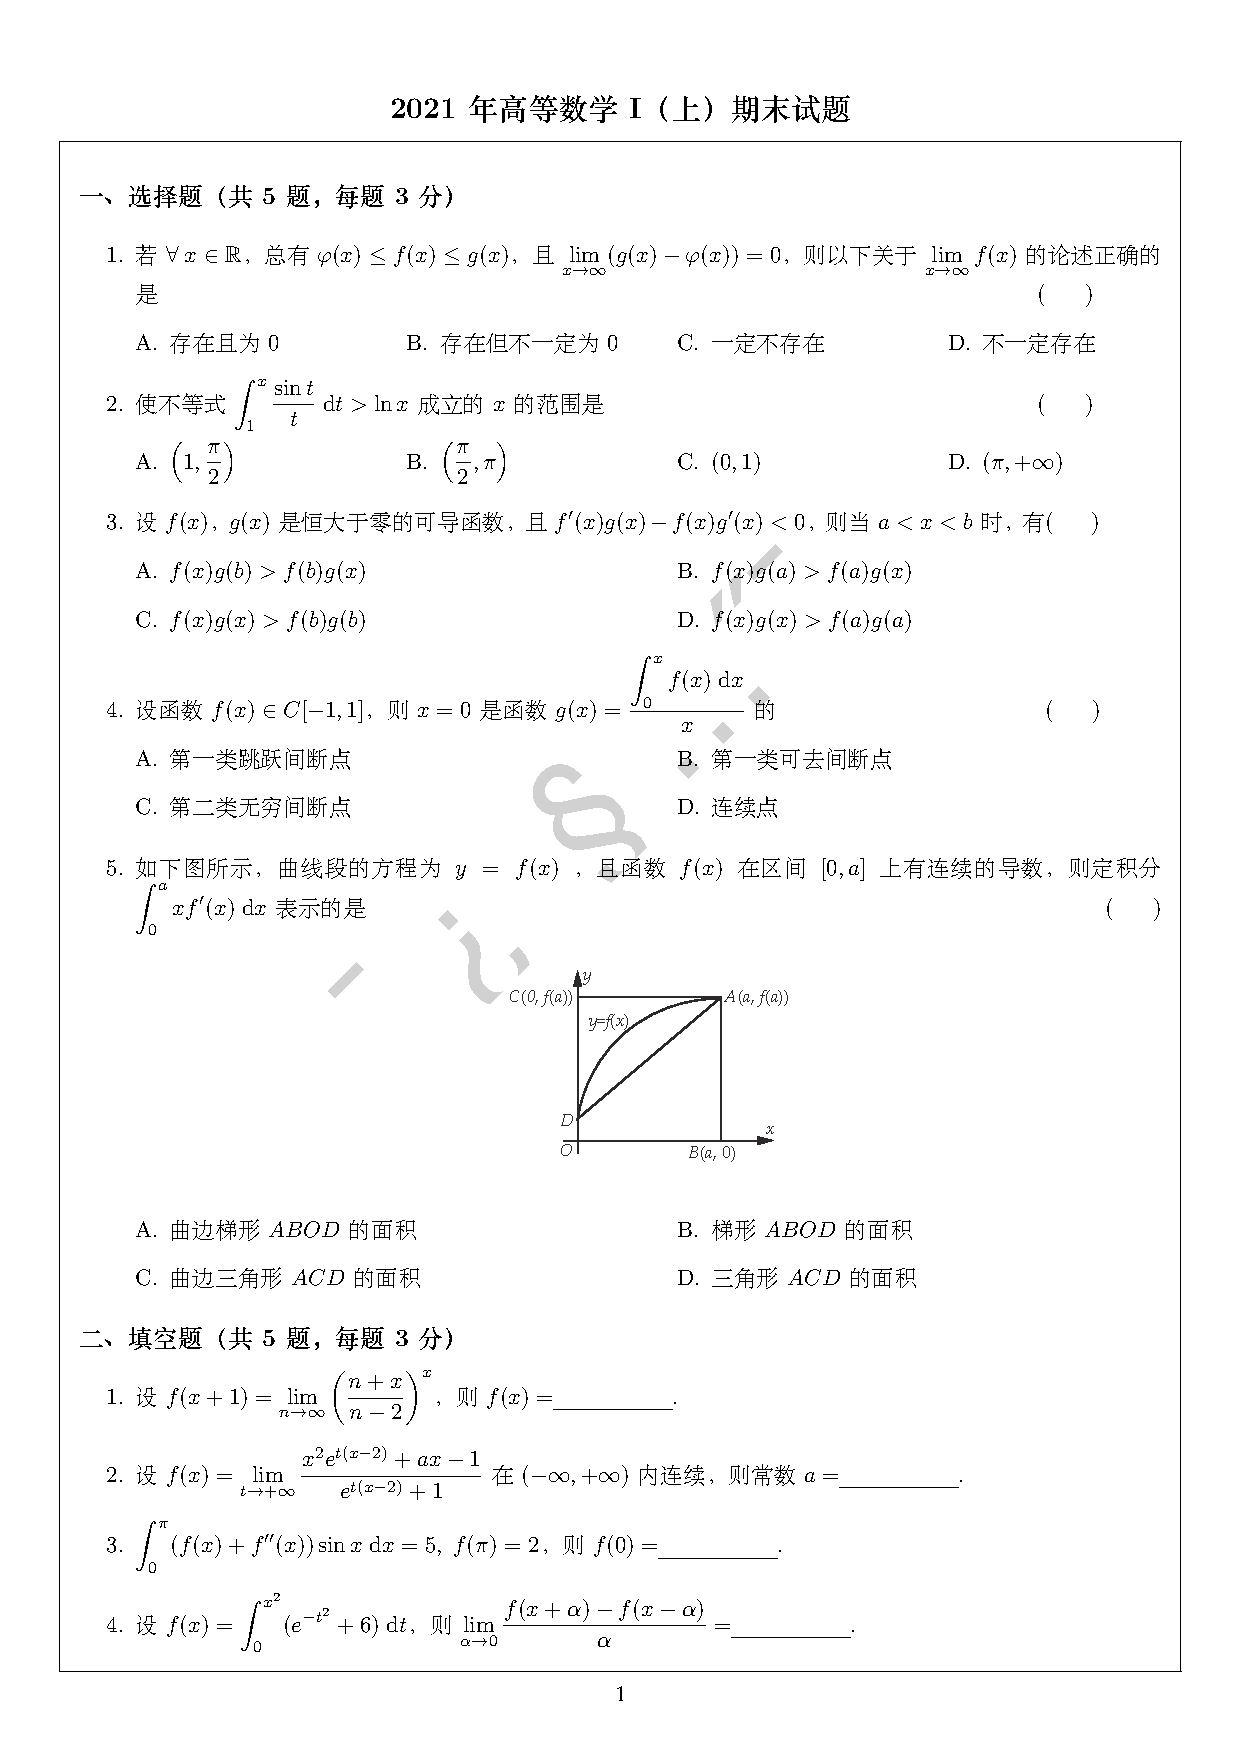
\includegraphics[scale=0.2]{figures/PK_GSZT.pdf}
                \end{figure}
            \end{column}
            \begin{column}{0.48\textwidth}
                \begin{figure}
                    \centering
                    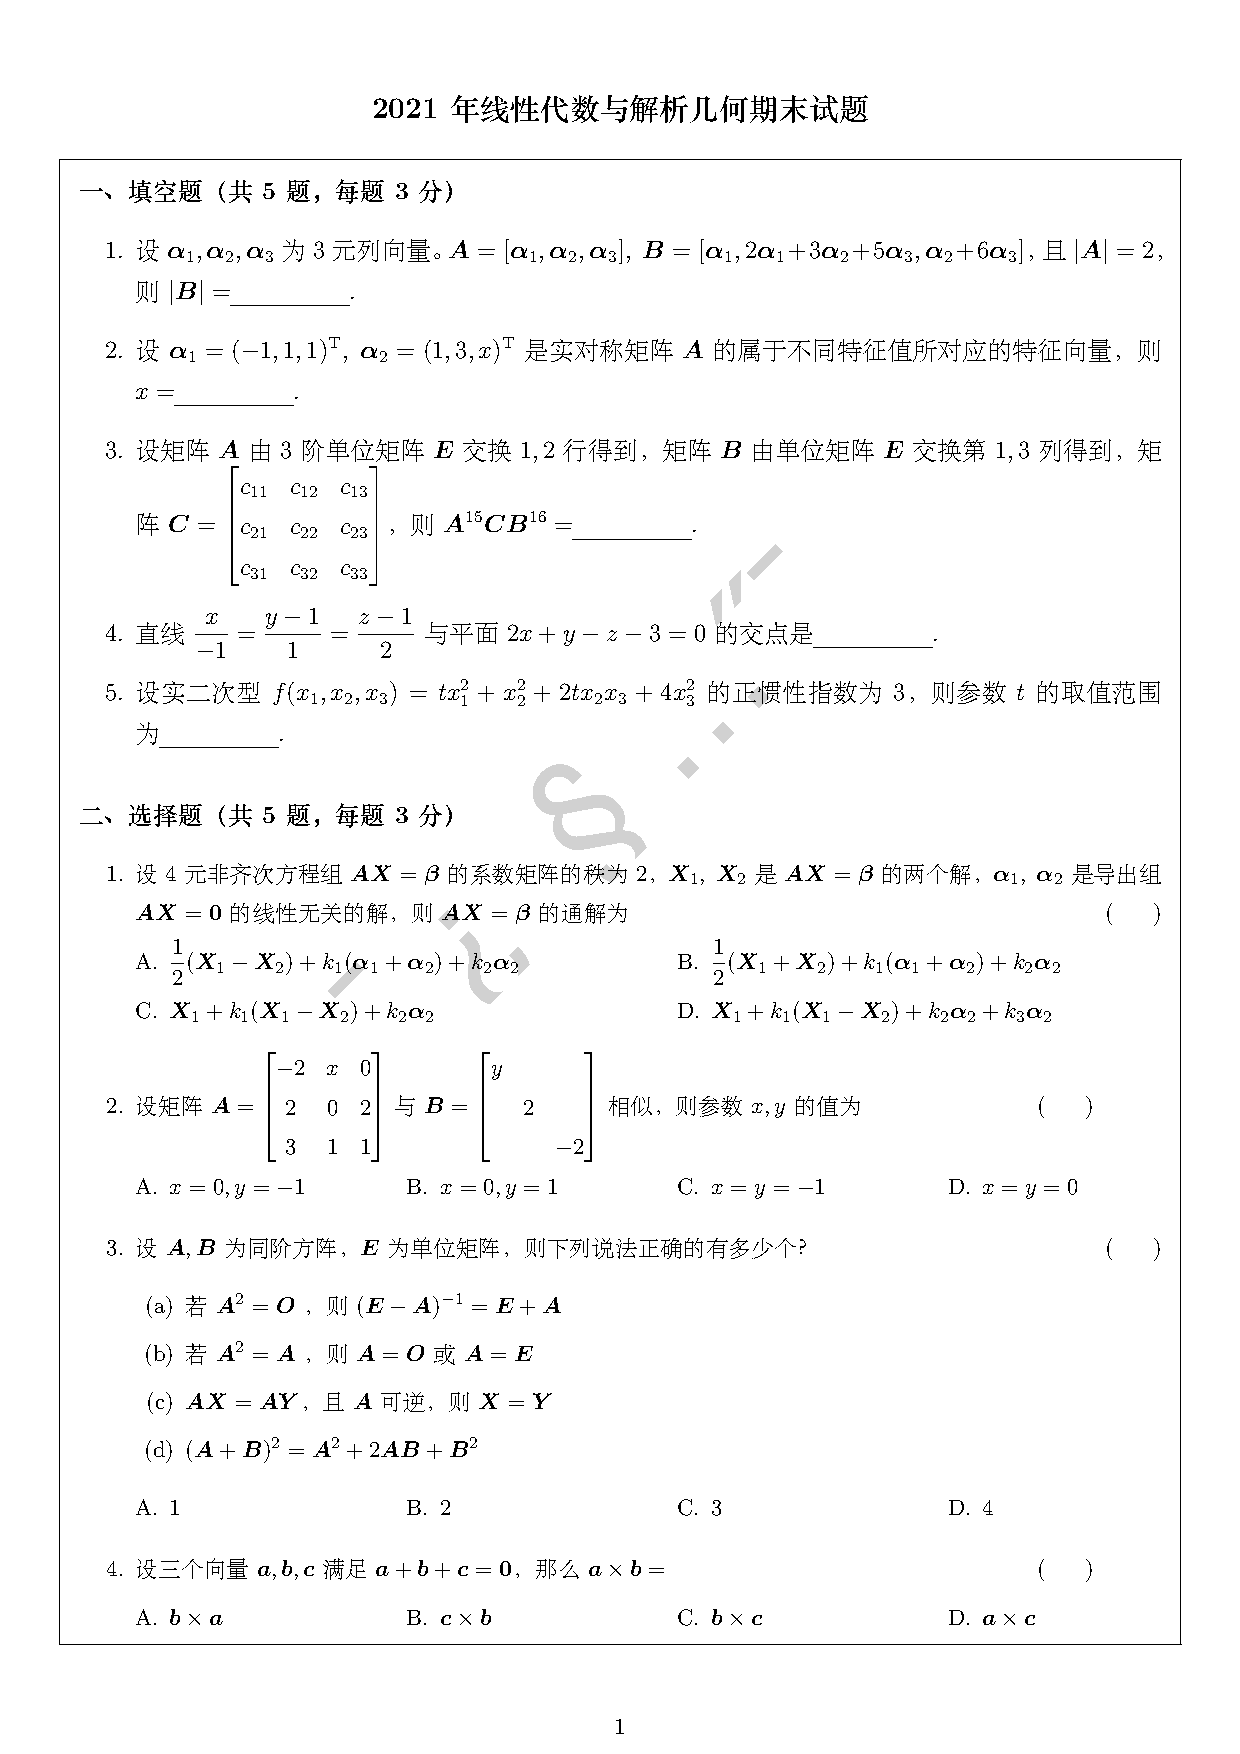
\includegraphics[scale=0.2]{figures/PK_XDZT.pdf}
                \end{figure}
            \end{column}
        \end{columns}
    \end{itemize}
\end{frame}